\documentclass{article}
\usepackage[a4paper, margin=1in]{geometry}
\usepackage[T1]{fontenc}
\usepackage[utf8]{inputenc}
\usepackage{amsmath, amssymb, graphicx, hyperref}
\usepackage{bookmark}
\graphicspath{{../figures/}}
\usepackage{bookmark}
\usepackage[framed,numbered]{matlab-prettifier}
\usepackage{xcolor}
\usepackage{listings}

\geometry{a4paper, margin=1in}

% MATLAB code style
\lstset{
  style      = Matlab-editor,
  basicstyle = \mlttfamily,
  breaklines = true
}

\title{\textbf{{Practical - 9}}}
\author{}
\date{October 24, 2026}

\pagenumbering{gobble}

\begin{document}
\maketitle

\noindent
\textbf{\large{Aim:}} To study the limited (logistic) growth of a population with and without harvesting.

\vspace{1em}
\noindent
\textbf{\large{Theory:}}

\noindent
\underline{Real Life Problem:} Suppose we have a population of fish in a lake. Initially, the number of fish increases because fish reproduce. 

\noindent
But the population cannot keep increasing forever because:
\begin{enumerate}
\item food is limited
\item space is limited
\item competition increases
\item resources become insufficient
\end{enumerate}
Therefore, the population eventually approaches a maximum sustainable population called the carrying capacity. This is called the logistic growth model.

\vspace{1em}
\begin{center}
    \textbf{\underline{Logistic Growth Model - Without Harvesting}}
\end{center}
\[\frac{dP}{dt} = rP(1 - \frac{P}{K})\]
\begin{itemize}
    \item $P(t) =$ population at time $t$
    \item $r =$ intrinsic growth rate
    \item $K =$ carrying capacity
    \item $t =$ time
\end{itemize}
\noindent\fbox{%
    \parbox{0.95\textwidth}{%
        \textbf{Note:}
        \begin{enumerate}
            \item $rP$ represents population growth
            \item The factor $(1 - \frac{P}{K})$ represents the effect of the carrying capacity on the population growth.
        \end{enumerate}
    }
}

\vspace{1em}

Three cases,
\begin{enumerate}
    \item If $P < K$, the population increases. 
    \item If $P = K$, the population stops increasing.
    \item If $P > K$, the population decreases towards K.
\end{enumerate}

\underline{Example:}
\begin{align*}
    P(0) &= 1000, \\
    r &= 0.1, \\
    K &= 10000, \\
    \frac{dP}{dt} &= 0.1P\left(1 - \frac{P}{10000}\right), \\
    P(0) &= 100.
\end{align*}

\noindent
\textbf{What graph will show?}

\noindent
The graph will start at 
$$P(0) = 1000$$ and increase.

\noindent
Initially, the population grows relatively quickly. 

\noindent
As $P$ gets closer to $K = 1000$, growth becomes slower.

\noindent
Finally, $$P(t) \rightarrow 1000$$
So the graph has an \textbf{S-shaped (sigmoid) curve}. 

\noindent
Therefore, the idea is population approaches carrying capacity rather than increasing indefinitely.
\vspace{2em}

\begin{center}
    \textbf{\underline{Logistic Growth Model - with Harvesting}}
\end{center}

Suppose humans catch some fish from the lake.

Let $H = $ Harvesting rate

\[\frac{dP}{dt} = rP(1 - \frac{P}{K}) - H\]

Here,
\begin{enumerate}
    \item $rP(1 - \frac{P}{K}) =$ Natural population growth
    \item $-H =$ fish being removed 
\end{enumerate}


\textit{Example -} With Harvesting
Take,
\begin{eqnarray*}
    r &=& 0.1, \\
    K &=& 10000, \\
    P(0) &=& 1000, \\
    H &=& 85, \\
    \frac{dP}{dt} &=& 0.1P(1 - \frac{P}{10000}) - 20, \\
    P(0) &=& 100.
\end{eqnarray*}

\newpage
\noindent
\textbf{\large{MATLAB Code:}}

\begin{lstlisting}
clc; clear all; close all;

syms P(t)

r = 0.1;
K = 10000;
P0 = 1000;
h = 85;

% Without Harvesting

eqn1 = diff(P,t) == r*P*(1-P/K);

init1 = P(0) == P0;

PSol1 = dsolve(eqn1,init1);

% With Harvesting

eqn2 = diff(P,t) == r*P*(1-P/K) - h;

init2 = P(0) == P0;

PSol2 = dsolve(eqn2,init2);

% Graph Plotting

disp(PSol1);
disp(PSol2);

fplot(PSol1, [0,200], 'LineWidth',2, color='r')

hold on

fplot(PSol2, [0,200], 'LineWidth',2, color='b')

grid on
xlabel('Time')
ylabel('Population')
title('Limited Population Growth with and without Harvesting')
legend('Without Harvesting', 'With Harvesting')


\end{lstlisting}

\vspace{3em}

\noindent
\textbf{\large{Output:}}

\vspace{0.5em}

\begin{flushleft}
$\frac{10000}{{\mathrm{e}}^{\log \left(9\right)-\frac{t}{10}} +1}$
\end{flushleft}
\begin{flushleft}
$500\,\sqrt{66}\,\tanh \left(\frac{\sqrt{66}\,{\left(33\,t-100\,\sqrt{66}\,\mathrm{atanh}\left(\frac{4\,\sqrt{66}}{33}\right)\right)}}{6600}\right)+5000$
\end{flushleft}

\vspace{0.5em}

\begin{figure}[htbp]
    \centering
    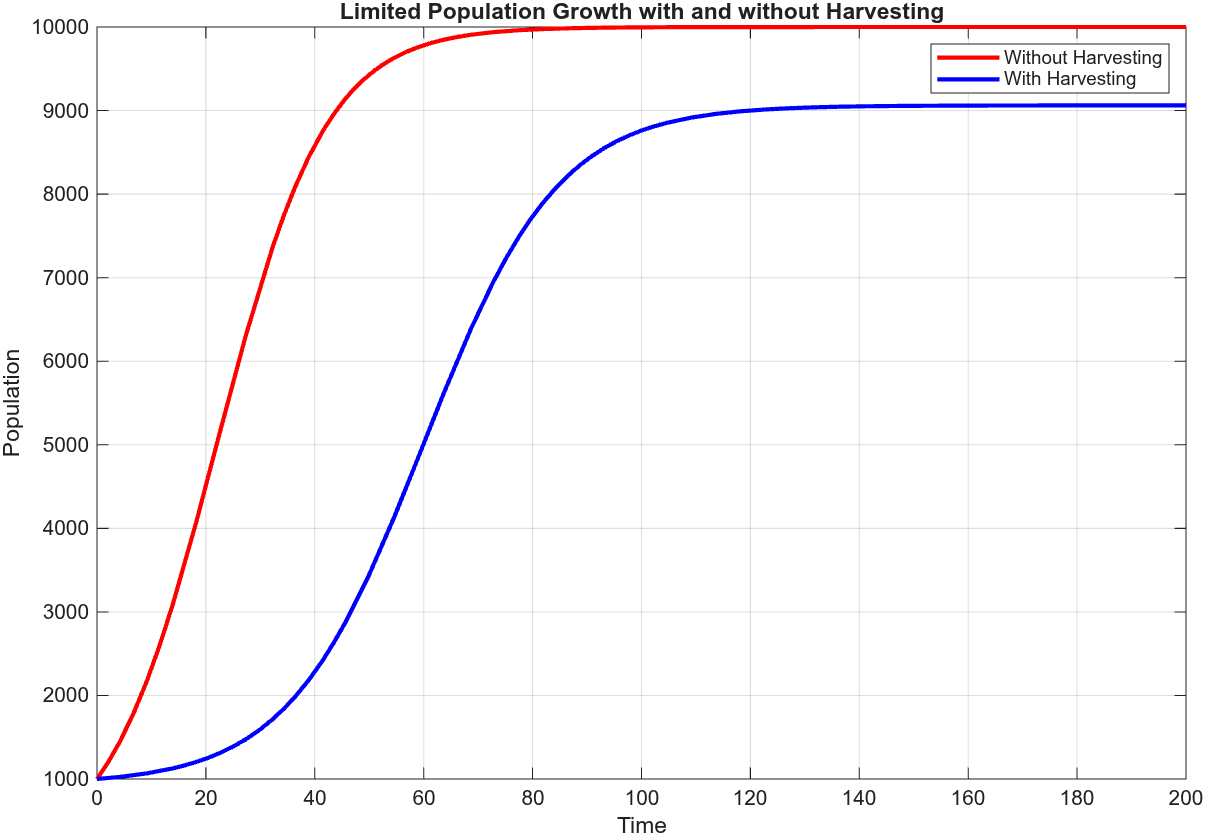
\includegraphics[width=0.7\textwidth]{Figure9.png}
\end{figure}


\newpage
\noindent
\textbf{\large{Observation:}}

\noindent
\underline{Without Harvesting:} $P(t) \rightarrow K$ so the population approaches 1000.

\noindent
\underline{With Harvesting:} The population settles at a lower level because fish are continuously being removed.

\end{document}
